\documentclass{beamer}

\usetheme[secheader]{Boadilla}
\setbeamertemplate{footline} {
  %\leavevmode%
  \hbox{%
  \begin{beamercolorbox}[wd=.5\paperwidth,ht=2.25ex,dp=1ex,left]{author in head/foot}%
    \usebeamerfont{author in head/foot}\hspace*{2ex}\insertshortauthor~~(adraeger@cern.ch)
  \end{beamercolorbox}%
  \begin{beamercolorbox}[wd=.5\paperwidth,ht=2.25ex,dp=1ex,right]{date in head/foot}%
    \usebeamerfont{date in head/foot}\insertshorttitle,~
    \insertshortdate{}\hspace*{1em}
    \insertframenumber{} / \inserttotalframenumber\hspace*{2ex}
  \end{beamercolorbox}}%
  \vskip0pt%
}
\beamertemplatenavigationsymbolsempty

\usepackage[percent]{overpic}
\usepackage{tikz}
%\usetikzlibrary{positioning,fit,shapes.arrows,shapes.geometric,shapes.misc,shapes.multipart,calc,shadows}
\tikzstyle{every picture}+=[remember picture]
\usepackage{booktabs}
\usepackage{graphicx}
\usepackage{rotating}
\usepackage{wasysym}
\usepackage{marvosym}
\graphicspath{{../../logo/}{figures/}{../../graphic-common/}}

\usepackage{amsmath}
\usepackage{cancel}
\usepackage{xspace}
\usepackage{xcolor}

% editing
\newcommand{\todo}[1]{\textcolor{red}{{\textbf{TODO: }\textit{#1}}}}
\newcommand{\fixme}[1]{\textcolor{red}{{\textbf{FIXME: }\textit{#1}}}}

% helpers
\newcommand{\emptybox}[1]{\parbox[c][#1]{0pt}{}}

% boxes
\newcommand{\cfbox}[2]{{\color{#1}\fbox{\normalcolor#2}}}

% Sectioning
\newcommand{\qsec}[1]{Section~\ref{#1}}
\newcommand{\qfig}[1]{Fig.~\ref{#1}}
\newcommand{\qtab}[1]{Table~\ref{#1}}
\newcommand{\qeq}[1]{\eqref{#1}}

% Particles
\newcommand{\W}{\ensuremath{\text{W}}\xspace}
\newcommand{\Z}{\ensuremath{\text{Z}}\xspace}

% Processes
\newcommand{\ZInv}{\ensuremath{\text{Z}\rightarrow\nu\bar{\nu}}\xspace}
\newcommand{\ZInvJets}{\ensuremath{\text{Z}\rightarrow\nu\bar{\nu}\,+\,\text{jets}}\xspace}
\newcommand{\Zmumu}{\ensuremath{\text{Z}\rightarrow\mu\bar{\mu}}\xspace}
\newcommand{\Zll}{\ensuremath{\text{Z}\rightarrow\text{ll}}\xspace}
\newcommand{\Zee}{\ensuremath{\text{Z}\rightarrow\text{ee}}\xspace}
\newcommand{\ttbar}{\ensuremath{\text{t}\bar{\text{t}}}\xspace}
\newcommand{\bbbar}{\ensuremath{\text{b}\bar{\text{b}}}\xspace}
\newcommand{\ccbar}{\ensuremath{\text{c}\bar{\text{c}}}\xspace}
\newcommand{\wpj}{\ensuremath{\text{W}+\text{jets}}\xspace}
\newcommand{\photonJet}{\ensuremath{\gamma+\text{jet}}\xspace}
\newcommand{\photonJets}{\ensuremath{\gamma+\text{jets}}\xspace}
\newcommand{\ZJet}{\ensuremath{\text{Z}+\text{jet}}\xspace}
\newcommand{\ZJets}{\ensuremath{\text{Z}+\text{jets}}\xspace}
\newcommand{\photonZJet}{\ensuremath{\text{photon}/Z+\text{jet}}\xspace}
\newcommand{\muonJets}{\ensuremath{\mu+\text{jets}}\xspace}

% Units
\newcommand{\tev}{\ensuremath{\;\text{Te}\kern-0.06667em\text{V}}\xspace}
\newcommand{\gev}{\ensuremath{\;\text{Ge}\kern-0.06667em\text{V}}\xspace}
\newcommand{\gevbrackets}{\ensuremath{\;[\text{Ge}\kern-0.06667em\text{V}]}\xspace}
\newcommand{\mev}{\ensuremath{\;\text{Me}\kern-0.06667em\text{V}}\xspace}
\newcommand{\kev}{\ensuremath{\;\text{ke}\kern-0.06667em\text{V}}\xspace}
\newcommand{\ev}{\ensuremath{\;\text{e}\kern-0.06667em\text{V}}\xspace}
\newcommand{\km}{\ensuremath{\;\text{km}}\xspace}
\newcommand{\m}{\ensuremath{\;\text{m}}\xspace}
\newcommand{\cm}{\ensuremath{\;\text{cm}}\xspace}
\newcommand{\mm}{\ensuremath{\;\text{mm}}\xspace}
\newcommand{\mum}{\ensuremath{\;\mu\text{m}}\xspace}
\newcommand{\hour}{\ensuremath{\;\text{h}}\xspace}
\newcommand{\second}{\ensuremath{\;\text{s}}\xspace}
\newcommand{\ns}{\ensuremath{\;\text{ns}}\xspace}
\newcommand{\kg}{\ensuremath{\;\text{kg}}\xspace}
\newcommand{\tons}{\ensuremath{\;\text{t}}\xspace}
\newcommand{\tesla}{\ensuremath{\;\text{T}}\xspace}
\newcommand{\kelvin}{\ensuremath{\;\text{K}}\xspace}
\newcommand{\nbinv}{\ensuremath{\;\text{nb}^{-1}}\xspace}
\newcommand{\pbinv}{\ensuremath{\;\text{pb}^{-1}}\xspace}
\newcommand{\fbinv}{\ensuremath{\;\text{fb}^{-1}}\xspace}
\newcommand{\pb}{\ensuremath{\;\text{pb}}\xspace}
\newcommand{\fb}{\ensuremath{\;\text{fb}}\xspace}
\newcommand{\mb}{\ensuremath{\;\text{mb}}\xspace}
\newcommand{\Hz}{\ensuremath{\;\text{Hz}}\xspace}

\newcommand{\gevnospace}{\ensuremath{\text{Ge}\kern-0.06667em\text{V}}\xspace}
\newcommand{\tevnospace}{\ensuremath{\text{Te}\kern-0.06667em\text{V}}\xspace}

% Quantities
\newcommand{\et}{\ensuremath{E_{\text{T}}}\xspace}
\newcommand{\met}{\ensuremath{\slash\mkern-12mu{E}_{\text{T}}}\xspace}
\newcommand{\metvec}{\ensuremath{\slash\mkern-12mu{\vec{E}}_{\text{T}}}\xspace}
\newcommand{\jetht}{\ensuremath{H_{\text{T}}}\xspace}
\newcommand{\mht}{\ensuremath{\slash\mkern-12mu{H}_{\text{T}}}\xspace}
\newcommand{\HT}{\ensuremath{H_{\text{T}}}\xspace}
\newcommand{\MHT}{\ensuremath{\slash\mkern-12mu{H}_{\text{T}}}\xspace}
\newcommand{\pt}{\ensuremath{p_{\text{T}}}\xspace}
\newcommand{\ptsup}[1]{\ensuremath{p^{#1}_{\text{T}}}\xspace}
\newcommand{\ptvec}{\ensuremath{\vec{p}_{\text{T}}}\xspace}
\newcommand{\ptvecsup}[1]{\ensuremath{\vec{p}^{#1}_{\text{T}}}\xspace}
\newcommand{\pti}[1]{\ensuremath{p_{\text{T},#1}}\xspace}
\newcommand{\ptivec}[1]{\ensuremath{\vec{p}_{\text{T},#1}}\xspace}
\newcommand{\ptjeti}[1]{\ensuremath{p^{\text{jet#1}}_{\text{T}}}\xspace}
\newcommand{\ptsub}[1]{\ensuremath{p_{\text{T},#1}}\xspace}
\newcommand{\ptvecsub}[1]{\ensuremath{\vec{p}_{\text{T},#1}}\xspace}
\newcommand{\ptdijet}{\ensuremath{p^{\text{dijet}}_{\text{T}}}\xspace}
\newcommand{\ptave}{\ensuremath{p^{\text{ave}}_{\text{T}}}\xspace}
\newcommand{\ptavemin}{\ensuremath{p^{\text{ave,min}}_{\text{T}}}\xspace}
\newcommand{\ptavemax}{\ensuremath{p^{\text{ave,max}}_{\text{T}}}\xspace}
\newcommand{\ptgen}{\ensuremath{p^{\text{gen}}_{\text{T}}}\xspace}
\newcommand{\ptgenave}{\ensuremath{p^{\text{gen,ave}}_{\text{T}}}\xspace}
\newcommand{\ptgenrel}{\ensuremath{p^{\text{gen,rel}}_{\text{T,3}}}\xspace}
\newcommand{\ptgeni}[1]{\ensuremath{p^{\text{gen}}_{\text{T},#1}}\xspace}
\newcommand{\pthat}{\ensuremath{\hat{p}_{\text{T}}}\xspace}
\newcommand{\pthatmin}{\ensuremath{\hat{p}^{\text{min}}_{\text{T}}}\xspace}
\newcommand{\pthatmax}{\ensuremath{\hat{p}^{\text{max}}_{\text{T}}}\xspace}
\newcommand{\pttrue}{\ensuremath{p^{\text{true}_{}}_{\text{T}}}\xspace}
\newcommand{\pttruei}[1]{\ensuremath{p^{\text{true}_{}}_{\text{T,}#1}}\xspace}
\newcommand{\ptmeas}{\ensuremath{p^{\text{meas}_{}}_{\text{T}}}\xspace}
\newcommand{\ptmeasi}[1]{\ensuremath{p^{\text{meas}_{}}_{\text{T,}#1}}\xspace}
\newcommand{\ptreco}{\ensuremath{p^{\text{reco}_{}}_{\text{T}}}\xspace}
\newcommand{\ptrel}{\ensuremath{\alpha}\xspace}
\newcommand{\ptrelmax}{\ensuremath{\alpha_{\text{max}}}\xspace}
\newcommand{\ptmin}{\ensuremath{p^{\text{min}_{}}_{\text{T}}}\xspace}
\newcommand{\ptmax}{\ensuremath{p^{\text{max}_{}}_{\text{T}}}\xspace}
\newcommand{\ptcalo}{\ensuremath{p^{\text{calo}_{}}_{\text{T}}}\xspace}
\newcommand{\ptcaloi}[1]{\ensuremath{p^{\text{calo}_{}}_{\text{T},#1}}\xspace}
\newcommand{\ptparticle}{\ensuremath{p^{\text{particle}_{}}_{\text{T}}}\xspace}
\newcommand{\ptparton}{\ensuremath{p^{\text{parton}_{}}_{\text{T}}}\xspace}
\newcommand{\ptref}{\ensuremath{p^{\text{ref}_{}}_{\text{T}}}\xspace}
\newcommand{\ppgen}{\ensuremath{p^{\text{gen}}_{||}}\xspace}
\newcommand{\ppgeni}[1]{\ensuremath{p^{\text{gen}}_{||,#1}}\xspace}
\newcommand{\pp}{\ensuremath{p_{||}}\xspace}
\newcommand{\ppi}[1]{\ensuremath{p_{||,#1}}\xspace}
\newcommand{\ppirel}[1]{\ensuremath{p^{\text{rel}}_{||,#1}}\xspace}
\newcommand{\etajeti}[1]{\ensuremath{\eta^{\text{jet#1}}}\xspace}
\newcommand{\etamin}{\ensuremath{\eta^{\text{min}}}\xspace}
\newcommand{\etamax}{\ensuremath{\eta^{\text{max}}}\xspace}
\newcommand{\fasym}{\ensuremath{f_{\text{Asym}}}\xspace}
\newcommand{\fasymdata}{\ensuremath{f^{\text{Data}}_{\text{Asym}}}\xspace}
\newcommand{\fasymmc}{\ensuremath{f^{\text{MC}}_{\text{Asym}}}\xspace}
\newcommand{\fresp}{\ensuremath{f_{\text{Resp}}}\xspace}
\newcommand{\alphat}{\ensuremath{\alpha_{\text{T}}}\xspace}
\newcommand{\resp}{\ensuremath{\mathcal{R}}\xspace}
\newcommand{\respmctruth}{\ensuremath{\mathcal{R}_{\text{MC}}}\xspace}
\newcommand{\sigmatruth}{\ensuremath{\sigma_{\text{MC}}}\xspace}
\newcommand{\asym}{\ensuremath{\mathcal{A}}\xspace}
\newcommand{\datasimratio}{\ensuremath{\rho}\xspace}
\newcommand{\NJets}{\ensuremath{N(\text{jets})}\xspace}
\newcommand{\BTag}{\ensuremath{B(\text{tags})}\xspace}
\newcommand{\Mass}[1]{\ensuremath{\text{M}_{\text{#1}}\xspace}}
\newcommand{\mass}[1]{\ensuremath{\text{m}_{\text{#1}}\xspace}}
\newcommand{\mtw}{\ensuremath{m_{T}(\text{W})\xspace}}
\newcommand{\mt}{\ensuremath{m_{T}\xspace}}
\newcommand{\deltaphi}{\ensuremath{\Delta\phi}}
\newcommand{\mindeltaphi}{\ensuremath{\Delta\phi_{N}^{min}}}
\newcommand{\deltaR}{\ensuremath{\Delta R}}
\newcommand{\hadtau}{\ensuremath{\tau_{\text{Had}\xspace}}}

% Symbols
\newcommand{\dif}[1]{\ensuremath{\text{d}#1}\xspace}
\newcommand{\e}{\,\text{e}}
\newcommand{\nup}[1]{$^{\text{\scriptsize #1}}$}
\newcommand{\dgr}{\ensuremath{\,^{\circ}}}
\newcommand{\mean}[1]{\ensuremath{\langle#1\rangle}}
\newcommand{\gqq}[1]{\ensuremath{\glqq#1\grqq}}
\newcommand{\rarr}{\ensuremath{\rightarrow}\xspace}

% Words and characters
\newcommand{\sm}{SM\xspace}
\newcommand{\diagonalsout}[1]{\ensuremath{\cancel{\text{#1}}}}
\newcommand{\genjet}{GenJet\xspace}
\newcommand{\genjets}{GenJets\xspace}
\newcommand{\calojet}{CaloJet\xspace}
\newcommand{\calojets}{CaloJets\xspace}
\newcommand{\window}[2]{\ensuremath{#1-#2\,\sigma}}
\newcommand{\windowinf}[1]{\ensuremath{#1\,\sigma - \infty}}
\newcommand{\pythia}{\textsc{Pythia}\xspace}
\newcommand{\pythiasix}{\textsc{Pythia6}\xspace}
\newcommand{\herwigpp}{\textsc{Herwig++}\xspace}
\newcommand{\herwig}{\textsc{Herwig}\xspace}
\newcommand{\madgraph}{\textsc{Madgraph}\xspace}
\newcommand{\CL}{C.\,L.\xspace}

% Jet related
\newcommand{\antikt}{anti-$k_{\text{T}}$\xspace}

% SUSY related
\newcommand{\susy}{SUSY\xspace}
\newcommand{\mssm}{MSSM\xspace}
\newcommand{\cmssm}{cMSSM\xspace}
\newcommand{\pmssm}{pMSSM\xspace}
\newcommand{\lsp}{LSP\xspace}
\newcommand{\mzero}{\ensuremath{m_{0}}\xspace}
\newcommand{\monehalf}{\ensuremath{m_{1/2}}\xspace}
\newcommand{\squark}{\ensuremath{\tilde{q}}\xspace}
\newcommand{\gluino}{\ensuremath{\tilde{g}}\xspace}
\newcommand{\msquark}{\ensuremath{m_{\tilde{q}}}\xspace}
\newcommand{\mgluino}{\ensuremath{m_{\tilde{g}}}\xspace}
\newcommand{\mneutralino}{\ensuremath{m_{\tilde{\chi}^{0}}}\xspace}
\newcommand{\tanbeta}{\ensuremath{\tan\beta}\xspace}
\newcommand{\stau}{\ensuremath{\tilde{\tau}}\xspace}
\newcommand{\neutralino}{\ensuremath{\tilde{\chi}^{0}}\xspace}

% Higgs related
\newcommand{\phitobb}{\ensuremath{\Phi\rightarrow\text{b}\bar{\text{b}}}\xspace}
\newcommand{\mhiggs}{\ensuremath{m_{\text{H}}}\xspace}
\newcommand{\mA}{\ensuremath{m_{\text{A}}}\xspace}
\newcommand{\mh}{\ensuremath{m_{\text{h}}}\xspace}
\newcommand{\mH}{\ensuremath{m_{\text{H}}}\xspace}
\newcommand{\mPhi}{\ensuremath{M_{\Phi}}\xspace}
\newcommand{\btageff}{\ensuremath{\epsilon(\text{b-tag})}\xspace}
\newcommand{\mjj}{\ensuremath{M_{12}}\xspace}
\newcommand{\xjjj}{\ensuremath{X_{123}}\xspace}
\newcommand{\mhmax}{\ensuremath{m^{\text{max}}_{h}}\xspace}


% Abbrevations
\newcommand{\etc}{etc.\ }
\newcommand{\wrt}{w.\,r.\,t.\ }
\newcommand{\cf}{cf.\ }
\newcommand{\ie}{i.\,e.\ }
\newcommand{\siehe}{s.\ }
\newcommand{\zb}{z.\,B.\ }
\newcommand{\ca}{ca.\ }
\newcommand{\eg}{e.\,g.\ }
\newcommand{\vs}{vs.\ }
\newcommand{\NB}{N.\,B.\xspace}

% Misc
\newcommand{\solidline}[1]{\textcolor{#1}{---}}
\newcommand{\dashedline}[1]{\textcolor{#1}{- -}}
\newcommand{\opencircle}[1]{\textcolor{#1}{$\circ$}}
\newcommand{\solidcircle}[1]{\textcolor{#1}{$\bullet$}}
\newcommand{\solidsquare}[1]{\textcolor{#1}{\small $\blacksquare$}}
\newcommand{\solidtriangle}[1]{\textcolor{#1}{\small $\blacktriangle$}}
\newcommand{\opensquare}[1]{\textcolor{#1}{\small $\square$}}
\newcommand{\opentriangle}[1]{\textcolor{#1}{\small $\triangle$}}
\newcommand{\opendiamond}[1]{\textcolor{#1}{\small $\diamond$}}
\newcommand{\greencheck}{\textcolor{beamerGreen}{\ensuremath{\checkmark}}\xspace}
\newcommand{\bibbullet}{\includegraphics[width=1em]{../../graphic-common/eyeCandy/freehand-book.png}}

% Colours
\definecolor{beamerGreen}{rgb}{0,0.6,0}
\definecolor{darkGreen}{rgb}{0,0.6,0}
\definecolor{beamerYellow}{rgb}{1.,0.745,0}
\definecolor{gray}{rgb}{0.4,0.4,0.4}
\definecolor{darkgreen}{RGB}{000,100,000}
\definecolor{kGreen2}{RGB}{000,153,000}
\definecolor{theme_blue}{RGB}{051,051,178}
\definecolor{theme_blue_light}{HTML}{ADADE0}

\newcommand{\blue}[1]{\textcolor{blue}{#1}}
\newcommand{\themeblue}[1]{\textcolor{theme_blue}{#1}}
\newcommand{\red}[1]{\textcolor{red}{#1}}
\newcommand{\orange}[1]{\textcolor{orange}{#1}}
\newcommand{\green}[1]{\textcolor{green}{#1}}
\newcommand{\yellow}[1]{\textcolor{yellow}{#1}}
\newcommand{\white}[1]{\textcolor{white}{#1}}
\newcommand{\grey}[1]{\textcolor{gray}{#1}}
\newcommand{\link}[2]{\href{#1}{\textcolor{theme_blue}{\underline{#2}}}}

% Libre-Office colours
\definecolor{oochart2}{HTML}{FF420E}  % orange
\definecolor{oochart7}{HTML}{314004}  % dark green
\definecolor{oochart11}{RGB}{197,001,012} % dark red
\definecolor{oochart12}{RGB}{001,132,209} % light blue


% ROOT colors
\definecolor{kBlack}{HTML}{000000}
\definecolor{kRed}{HTML}{FF0000}
\definecolor{kRedUp2}{HTML}{6B0C0C}
\definecolor{kYellow}{HTML}{FEFE12}
\definecolor{kBlue}{HTML}{0000FF}
\definecolor{kOrange}{HTML}{FFCC00}
\definecolor{kGreen}{HTML}{59D454}
\definecolor{kGreenUp2}{HTML}{009900}
\definecolor{kMagenta}{HTML}{FF00FF}
\definecolor{kCyan}{HTML}{00FFFF}

\newcommand{\lib}[1]{\tiny #1}

% Title etc
\title[SUSY-Workshop]{\huge Status of RA2/b\vspace{0.5cm}}
\subtitle{\Large Background Estimation Methods:\\
\ZInvJets \\ \ttbar \& \wpj \\\vspace{0.1cm}
\large Isolated Track vs Isolated (light) Lepton Veto}
\author[Arne-Rasmus~Dr\"ager]{
  Arne-Rasmus~Dr\"ager (Uni Hamburg)\\on behalf of the RA2/b team
}
\date[October 31, 2014]{October 31, 2014
 % \vskip1cm
  \begin{center}
    
\includegraphics[height=1cm]{Universitaet-Hamburg-Logo.jpg}
    \hskip8cm
    
\includegraphics[height=1cm]{CMSlogo.jpeg}
  \end{center}
}

% pdflatex packages
\hypersetup{bookmarks=true}
\hypersetup{unicode=false}
\hypersetup{pdftitle={Status report of RA2/b Part B}}
\hypersetup{pdfauthor={Arne-Rasmus~Dr\"ager}}


\begin{document}
% ==================================================
% --------------------------------------------------
\section{Title}
\begin{frame}
  \titlepage
\end{frame}

% --------------------------------------------------

\section{RA2 RA2b joined effort}
\begin{frame}
\frametitle{Two analysis two strategies}
   \begin{columns}
    \begin{column}{0.5\textwidth}
     \large RA2
     \normalsize
     \begin{itemize}
      \item $\HT >500 \gev$ 
      \begin{itemize}
       \item Jets: $\pt>50\gev$, $|\eta|<2.5$
      \end{itemize}
      \item $\MHT >200 \gev$
            \begin{itemize}
       \item Jets: $\pt>30\gev$, $|\eta|<5.0$
      \end{itemize}
      \item $\NJets\ge 3$, $\pt>50\gev$
      \begin{itemize}
       \item Jets: Following \HT definition
      \end{itemize}

      \item $\deltaphi_{1,2,3}>0.5,0.5,0.3$
      \item Isolated electron \& muon veto
     \end{itemize}

    \end{column}
        \begin{column}{0.5\textwidth}
     \large RA2b
     \normalsize
             \begin{itemize}
      \item $\HT >400 \gev$ 
      \item $\met >0 \gev$
      \item Jet(1,2,3) $\pt>70,70,50\gev$
      \item $\BTag\ge1$ CSVM ($>0.679$) $\pt>30\gev$
      \item $\mindeltaphi>4$
      \item Isolated electron \& muon veto
     \end{itemize}
     
    \end{column}
\end{columns}

\begin{block}{}
\centering
\Large RA2/b having same main SM backgrounds\\
\end{block}
\end{frame}
% --------------------------------------------------

\section{Outline}

\begin{frame}
\frametitle{Studies of Background Estimation Methods \\ using 13\tev csa14 samples (25ns)}
\begin{columns}
 \begin{column}{0.5\textwidth}
  \begin{itemize}
   \item \ZInvJets events\\
   \begin{itemize}
    \item \Zll (Troy Mulholland)
    \item \photonJets (Andrew Whitbeck)
   \end{itemize}
   \vspace{10mm}
   \item \wpj \& \ttbar events
   \begin{itemize}
   \item Lost-Lepton Background
   \item Isolated Track
         \\(Arne-Rasmus Dr\"ager)
   \end{itemize}
   \end{itemize}
  \end{column}
   \begin{column}{0.5\textwidth}
      \begin{overpic}[width=0.70\textwidth]{figures/ZInvis.png}\end{overpic}
      \\
      \vspace{5mm}
      \begin{overpic}[width=0.70\textwidth]{figures/LostLepton.png}\end{overpic}
   \end{column}
\end{columns}
\end{frame}
% --------------------------------------------------
\section{\ZInvJets}
\begin{frame}
  \begin{center}
    \huge\ZInvJets
    
  \end{center}
\end{frame}
% --------------------------------------------------


\subsection{\Zll - Introduction}
\begin{frame}
\frametitle{Estimation of \ZInvJets  Using \Zll Events}
\begin{itemize}
 \item Main Idea: Remove four-momentum of reconstructed \Zll events in selection (except lepton veto). Recompute relevant quantities (e.q. \met, $\Delta\Phi_{N}^{min}$)
 \item Work flow:
 \begin{itemize}
  \item Correct for branching fraction ($R = 5.95$)
  \item Increase statistics of \Zll events by loosening b-jet tagger and applying a scale factor ($F$) to each b-jet bin
  \item Measure efficiency ($\epsilon$) of reconstructing \Zll event with a Tag\&Probe method
  \item Determine and correct for purity ($P$) of \Zll selection
  \item Apply lepton acceptance corrections ($A$)
 \end{itemize}
\end{itemize}
  \begin{centering}
  $\text{N }(\ZInv) = \text{N }(\Zll)\cdot F \cdot P \cdot R / (A\cdot \epsilon)$
  \end{centering}
  \begin{block}{}
\centering
% SAY: 2 ways to proceed
\end{block}
\end{frame}

% --------------------------------------------------
\subsection{Efficiencies using a Tag\&Probe method }
\begin{frame}
 \frametitle{Determination of lepton efficiencies}
 Move to backup if no time
\end{frame}


% --------------------------------------------------
\subsection{\Zll \met Closure}
\begin{frame}
 \frametitle{Normalized \met distribution for 0 and 1 CSVM b-jet}
 \begin{overpic}[width=0.95\textwidth]{figures/ZwithLepLep/MET_Closure.png}
	%\put(60,53){\rotatebox{0}{\scriptsize Pass}}
     \end{overpic}\\
 \begin{itemize}
  \item Leptons corrected for reconstruction efficiencies ($0.929 < \epsilon < 0.975$) and acceptance ($0.632 < A< 0.886$) 
 \end{itemize}

\end{frame}

% --------------------------------------------------
\subsection{\Zll Scaling of loose b-jet Region to tight Region}
\begin{frame}
 \frametitle{Scaling factor for b-jet regions}
 \begin{itemize}
  \item Increase statistics by loosen cut on b-taggger to CSVL scale using independent control sample (QCD \& MET/HT inverted DY)
 \end{itemize}
    \begin{columns}
    \begin{column}{0.5\textwidth}
     \begin{itemize}
      \item  8\tev QCD enriched sample agreed in data but not in MC
      \item Check will be done once data is availabe. For now inverted MET/HT DY samples used to calcuate scale factors
     \end{itemize}
           \Zee prediction using inverted MET/HT sample
           \begin{tabular}{|r|l|l|}
        \hline
        b-jets  & Prediction & Expectation \\ 
	1	& $840.3\pm 32.3$ & 834\\
	2	& $332.0\pm 18.8$ & 365\\
	3	& $15.71\pm 4.39$ & 16\\
        \hline
    \end{tabular}
    \end{column}
        \begin{column}{0.5\textwidth}
\begin{overpic}
       [width=0.95\textwidth]{figures/ZwithLepLep/CSV_Most_blikeJet.png}
      \end{overpic}
     
    \end{column}
\end{columns}
\end{frame}


% --------------------------------------------------
\subsection{\Zmumu -Efficiencies}
\begin{frame}
\frametitle{Comparison of $\mu$ efficiencies}
\centering
 $\met>400, \HT>1000$
   \begin{columns}
    \begin{column}{0.5\textwidth}
     \centering 8\tev (Data)
    \end{column}
        \begin{column}{0.5\textwidth}
        \centering 13\tev (MC)
     
    \end{column}
\end{columns}
  \begin{columns}
    \begin{column}{0.5\textwidth}
     \centering
      \begin{overpic}[width=0.70\textwidth]{figures/ZwithLepLep/8TeVZmm_pass.pdf}
	\put(60,53){\rotatebox{0}{\scriptsize Pass}}
     \end{overpic}\\
           \begin{overpic}[width=0.70\textwidth]{figures/ZwithLepLep/8TeVZmm_fail.pdf}
	      \put(60,53){\rotatebox{0}{\scriptsize Fail}}
     \end{overpic}\\
     
    \end{column}
    \begin{column}{0.5\textwidth}
      \centering
       \begin{overpic}[width=0.50\textwidth]{figures/ZwithLepLep/13TeVTightCutZmm_pass.pdf}
	 \put(68,75){\rotatebox{0}{\scriptsize Pass}}
	 \put(100,90){\rotatebox{-45}{\scriptsize \Large Troy}}
      \end{overpic}\\
       \begin{overpic}[width=0.50\textwidth]{figures/ZwithLepLep/13TeVTightCutZmm_fail.pdf}
	 \put(68,75){\rotatebox{0}{\scriptsize Fail}}
     \end{overpic}
    \end{column}
  \end{columns}
   \begin{columns}
    \begin{column}{0.5\textwidth}
     \centering Efficiency: $\epsilon = 0.870 \pm 0.028$
    \end{column}
        \begin{column}{0.5\textwidth}
        \centering Efficiency: $\epsilon = 0.930 \pm 0.010$
     
    \end{column}
\end{columns}
\end{frame}

% --------------------------------------------------

\subsection{\Zee -Efficiencies}
\begin{frame}
\frametitle{Comparison of electron efficiencies}
\centering
 $\met>400, \HT>1000$
   \begin{columns}
    \begin{column}{0.5\textwidth}
     \centering 8\tev (Data)
    \end{column}
        \begin{column}{0.5\textwidth}
        \centering 13\tev (MC)
     
    \end{column}
\end{columns}
  \begin{columns}
    \begin{column}{0.5\textwidth}
     \centering
      \begin{overpic}[width=0.70\textwidth]{figures/ZwithLepLep/8TeVZee_pass.pdf}
	\put(60,53){\rotatebox{0}{\scriptsize Pass}}
     \end{overpic}\\
           \begin{overpic}[width=0.70\textwidth]{figures/ZwithLepLep/8TeVZee_fail.pdf}
	     \put(60,53){\rotatebox{0}{\scriptsize Fail}}
     \end{overpic}\\
     
    \end{column}
    \begin{column}{0.5\textwidth}
      \centering
       \begin{overpic}[width=0.50\textwidth]{figures/ZwithLepLep/13TeVTightCutZee_pass.pdf}
	 \put(68,75){\rotatebox{0}{\scriptsize Pass}}
	 \put(100,90){\rotatebox{-45}{\scriptsize \Large Troy}}
      \end{overpic}\\
       \begin{overpic}[width=0.50\textwidth]{figures/ZwithLepLep/13TeVTightCutZee_fail.pdf}
	 \put(68,75){\rotatebox{0}{\scriptsize Fail}}
     \end{overpic}
    \end{column}
  \end{columns}
   \begin{columns}
    \begin{column}{0.5\textwidth}
     \centering Efficiency: $\epsilon =0.877 \pm 0.056$
    \end{column}
        \begin{column}{0.5\textwidth}
        \centering Efficiency: $\epsilon =0.957 \pm 0.008$
     
    \end{column}
\end{columns}
\end{frame}

% --------------------------------------------------

\subsection{\Zll}
\begin{frame}
\frametitle{Summary Progress \Zll}
 \begin{itemize}
  \item Tag \& Probe efficiencies for \Zll events have been determined for the relevant regions on the csa14 13\tev samples.
  \item Muon efficiencies:
  \begin{itemize}
  \item nominal cuts $\epsilon = 0.938 \pm 0.001$ ($\met > 125 \gev, \HT > 400 \gev $)
   \item tight cuts  $\epsilon = 0.930 \pm 0.010$ ( $\met > 400 \gev, \HT > 1000 \gev $)
  \end{itemize}
  \item Electron efficiencies:
  \begin{itemize}
  \item nominal cuts $\epsilon = 0.962 \pm0.001$ ($\met > 125 \gev, \HT > 400 \gev $)
   \item tight cuts  $\epsilon = 0.957 \pm 0.008$ ($\met > 400 \gev, \HT > 1000 \gev $)
  \end{itemize}
  \item Overall the 13\tev lepton reconstruction efficiencies are better in respect to 8\tev
 \end{itemize}

\end{frame}

% --------------------------------------------------
\subsection{\photonJets - Introduction}
\begin{frame}
\frametitle{\ZInv estimation using \photonJets events}
%\frametitle{Did We Discover the Standard-Model Higgs?}
\begin{itemize}
 \item Main Idea: Exploit kinematic similarities of Z/$\gamma$ at high boson \pt.
 \item Work flow:
 \begin{itemize}
  \item Remove $\gamma$ from event and recompute search variables
  \item Apply Z/$\gamma$ ratio correction parametrized in \MHT \& \NJets
  \item Correct for $\gamma$ acceptance and reconstruction efficiency ($\epsilon_{\text{ID/Iso}}$)
  \item Apply lepton acceptance corrections ($A$)
 \end{itemize}
\end{itemize}
  \begin{centering}
  $\text{N }(\ZInv) = \text{N }(\gamma)\cdot R(\ZInv/\gamma)\cdot P\xspace/ (A\cdot \epsilon_{\text{ID/Iso}})$
  \end{centering}
\begin{block}{}
\centering
% SAY: 2 ways to proceed
Study of photon (slimmedPhotons) $\epsilon_{\text{ID/Iso}}$ efficiencies using 13\tev miniAOD MC (50 ns BX \& 40 PU) at $\HT>400\gev$\\
Compare $\epsilon_{\text{ID/Iso}}$ efficiencies to 8\tev results
\end{block}

\end{frame}
\subsection{\photonJets - Photon ID}
\begin{frame}
%\frametitle{Comparison $\gamma$ properties}
   \begin{itemize}
    \item Photon ID variables:
   \end{itemize}
  \begin{columns}
   \begin{column}{0.33\textwidth}
     \begin{overpic}[width=0.8\textwidth]{figures/ZwithGamma/8_13Comp_hOverE-eps-converted-to.pdf} \end{overpic}
   \end{column}
   \begin{column}{0.33\textwidth}
     \begin{overpic}[width=0.8\textwidth]{figures/ZwithGamma/8_13Comp_pixelSeed-eps-converted-to.pdf} \end{overpic}
   \end{column}
   \begin{column}{0.33\textwidth}
     \begin{overpic}[width=0.8\textwidth]{figures/ZwithGamma/8_13Comp_sigmaIetaIeta-eps-converted-to.pdf} 
      \put(35,94){\rotatebox{0}{\scriptsize Barrel only}}
      \put(90,110){\rotatebox{-45}{\scriptsize \Large Andrew}}
      \end{overpic}

   \end{column}

  \end{columns}
  \begin{itemize}
   \item Isolation of photons passing ID requirements \& $p_{T}^{\gamma}>100\gev$
  \end{itemize}

    \begin{columns}
   \begin{column}{0.33\textwidth}
     \begin{overpic}[width=0.8\textwidth]{figures/ZwithGamma/8_13Comp_coneIsoCharged-eps-converted-to.pdf} \end{overpic}
   \end{column}
   \begin{column}{0.33\textwidth}
     \begin{overpic}[width=0.8\textwidth]{figures/ZwithGamma/8_13Comp_coneIsoNeutral-eps-converted-to.pdf} \end{overpic}
   \end{column}
   \begin{column}{0.33\textwidth}
     \begin{overpic}[width=0.8\textwidth]{figures/ZwithGamma/8_13Comp_coneIsoPhoton-eps-converted-to.pdf} \end{overpic}
   \end{column}

  \end{columns}

\end{frame}
\subsection{\photonJets - ID/Iso Selection}
\begin{frame}
\frametitle{Photon ID/Iso Selection 8\tev}
    \begin{columns}
   \begin{column}{0.33\textwidth}
  \begin{overpic}[width=1\textwidth]{figures/ZwithGamma/table.png} \end{overpic}
 \end{column}
 \begin{column}{0.66\textwidth}
   \begin{overpic}[width=1\textwidth]{figures/ZwithGamma/table2.png} \end{overpic}
 \end{column}
\end{columns}
\begin{itemize}
 \item Rho correction to the isolation variables applied \\
 $\text{ISO}_{\text{corr}} = \text{max}(\text{Iso} - \text{E}_{\text{A}} \cdot \rho , 0) $
 \item Same $\text{E}_{\text{A}}$ as for 8\tev analysis
\end{itemize}


\end{frame}






% --------------------------------------------------
\section{Lost-Lepton Background }
\begin{frame}
  \begin{center}
    \huge Lost-Lepton Background
    
  \end{center}
\end{frame}

\subsection{Basic concept}
\begin{frame}
  \frametitle{Mainly \ttbar and \wpj events where prompt electrons or muons are lost}
   \begin{figure}
 \centering
  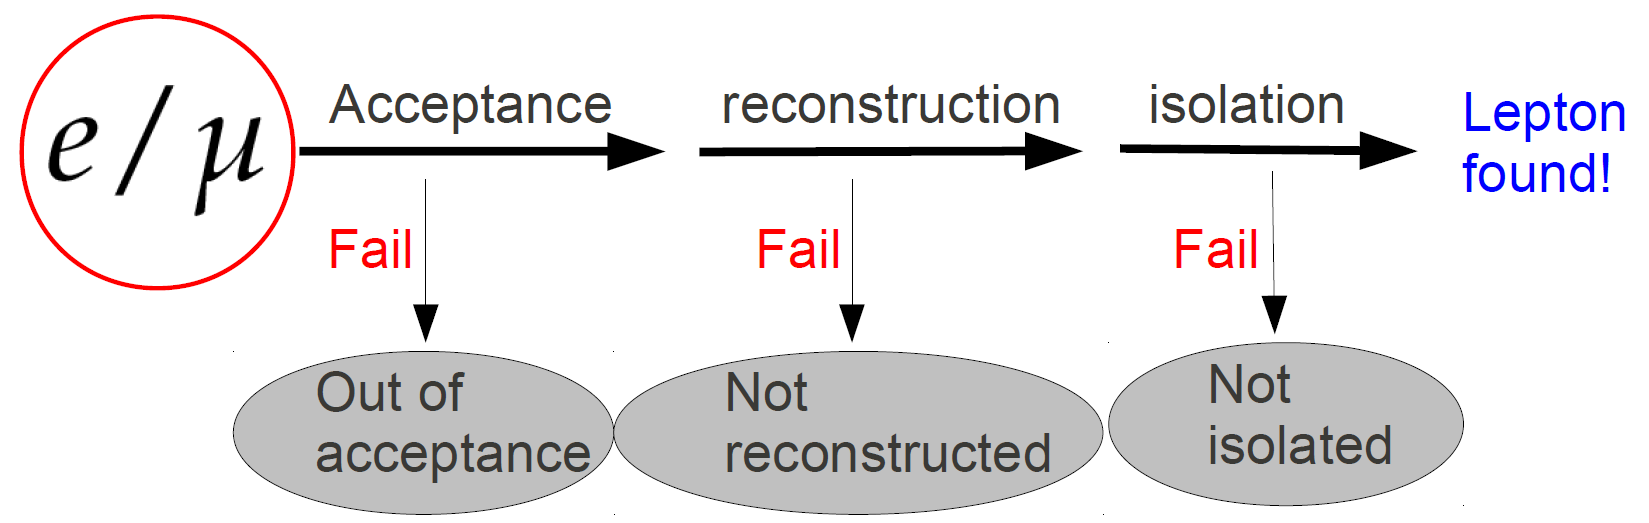
\includegraphics[width = 0.65\textwidth]{figures/lost-lepton/lepton_veto_sketch.png}
%  \caption{Awesome figure}
 \end{figure}
      \begin{itemize}
      \item Select a control sample (CS) of exactly one well isolated $\mu$ within the acceptance
        \begin{itemize}
        \item Weight each CS event according to efficiencies for each identification step (efficiencies determined from \ttbar and \wpj sample)
        \item Isolation and reconstruction efficiency in \HT, \MHT and \NJets parametrized
        \item Acceptance in \MHT and \NJets
        \end{itemize}
      \end{itemize}
\end{frame}
% --------------------------------------------------
\subsection{Muon Control Sample Corrections }
\begin{frame}
\begin{itemize}
 \item Signal and other SM processes can contribute to $\mu$ control sample
 \item Suppress contamination by requiring trans. mass $\mt < 100 \gev$ \\
\end{itemize}
\vspace{0.5cm}
$m_{T} = \sqrt{2 \cdot p_{T}(\mu)\cdot \met (1 - \cos(\Delta \Phi))}$

  \begin{columns}
    \begin{column}{0.4\textwidth}

      \begin{itemize}
      \item Removes about 15\% of $\mu$ CS due to:
        \begin{itemize}
        \item di-leptonic \ttbar decays
        \item Mismeasured jets
        \item Highly virtual W
        \end{itemize}
      \begin{centering}
      \end{centering}
      \item Correction as a function of \MHT, \NJets applied
      \end{itemize}
    \end{column}
    \begin{column}{0.6\textwidth}
      \centering
      \begin{overpic}[width=0.8\textwidth]{figures/lost-lepton/ControlSample__MTW__MCPrMTWDiLepTTbar+MCPrMTWDiLepW__mu_control_sample.pdf}
        \put(41.52,83){\color{black}\line(0,-1){67}}
	%\put(90,90){\rotatebox{-45}{\scriptsize \Large Arne}}
      \end{overpic}
    \end{column}
  \end{columns}
  \begin{itemize}
   \item Contribution of di leptonic \ttbar events ~3\% 
   \begin{itemize}
    \item Separate estimation leading to about ~1\% of total background
   \end{itemize}

  \end{itemize}

\end{frame}
% --------------------------------------------------

\subsection{Closure Test}
\begin{frame}

Closure test for the lost-lepton method:\\
\begin{itemize}
 \item $\HT > 500 \gev$ , $\MHT>100 \gev$, $\NJets\ge 3$ , $\Delta\Phi_{1,2,3}>$0.5, 0.5, 0.3
\end{itemize}
  \begin{columns}
    \begin{column}{0.5\textwidth}
     \centering
      \begin{overpic}[width=0.57\textwidth]{figures/lost-lepton/Closure__HT__MCPrMTWDiLep_vs_MCEx__csa_Baseline.pdf}
     \end{overpic}
           \begin{overpic}[width=0.57\textwidth]{figures/lost-lepton/Closure__NJets__MCPrMTWDiLep_vs_MCEx__csa_Baseline.pdf}
     \end{overpic}
    \end{column}
    \begin{column}{0.5\textwidth}
      \centering
            \begin{overpic}[width=0.57\textwidth]{figures/lost-lepton/Closure__MHT__MCPrMTWDiLep_vs_MCEx__csa_Baseline.pdf}
	 %     \put(90,90){\rotatebox{-45}{\scriptsize \Large Arne}}
     \end{overpic}
      \begin{overpic}[width=0.57\textwidth]{figures/lost-lepton/Closure__NVtx__MCPrMTWDiLep_vs_MCEx__csa_Baseline.pdf}
      \end{overpic}
    \end{column}
  \end{columns}
  \begin{itemize}
   \item Good agreement between expectation ($30462.9 \pm 60.0$) and prediction ($30128.1 \pm 80.9$) for all search variables
  \end{itemize}

\end{frame}
% --------------------------------------------------
\subsection{Closure Test: BTag}
\begin{frame}

Preliminary closure: Efficiencies binned in BTags instead of \NJets\\
\begin{itemize}
 \item $\HT > 500 \gev$ , $\MHT>100 \gev$, $\NJets\ge 3$ , $\Delta\Phi_{1,2,3}>$0.5, 0.5, 0.3
\end{itemize}

  \begin{columns}
    \begin{column}{0.5\textwidth}
     \centering
      \begin{overpic}[width=0.57\textwidth]{figures/lost-lepton/Closure__HT__MCPrMTWDiLepBTag_vs_MCEx__csa_Baseline.pdf}
     \end{overpic}
           \begin{overpic}[width=0.57\textwidth]{figures/lost-lepton/Closure__BTags__MCPrMTWDiLepBTag_vs_MCEx__csa_Baseline.pdf}
     \end{overpic}
    \end{column}
    \begin{column}{0.5\textwidth}
      \centering
            \begin{overpic}[width=0.57\textwidth]{figures/lost-lepton/Closure__MHT__MCPrMTWDiLepBTag_vs_MCEx__csa_Baseline.pdf}
	 %     \put(90,90){\rotatebox{-45}{\scriptsize \Large Arne}}
     \end{overpic}
      \begin{overpic}[width=0.57\textwidth]{figures/lost-lepton/Closure__NVtx__MCPrMTWDiLepBTag_vs_MCEx__csa_Baseline.pdf}
      \end{overpic}
    \end{column}
  \end{columns}
  \begin{itemize}
   \item Good closure \HT, \MHT and BTags\\ Exp: $30462.9 \pm 60.0$ pre: $31071.1  \pm 84.9$
  \end{itemize}

\end{frame}

% --------------------------------------------------
\section{Isolated Track vs Lepton Veto }
\begin{frame}
\frametitle{Isolated Track vs Isolated Electron \& Muon Lepton Veto}
  \begin{columns}
    \begin{column}{0.33\textwidth}
     \centering
      \begin{overpic}[width=0.95\textwidth]{figures/IsolatedTrack/rejection/IsoTrackStudies__HT__LeptonEx_vs_ITExW+ITExTTbar__Baseline_LeptonVeto_vs_IsoTrackVeto.pdf}
     \end{overpic}
           \begin{overpic}[width=0.95\textwidth]{figures/IsolatedTrack/purity/IsoTrackStudies__HT__LeptonEx_vs_ITExWTrue+ITExWFalse+ITExTTbarTrue+ITExTTbarFalse__Baseline_LeptonVeto_vs_IsoTrackVeto_purity.pdf}
     \end{overpic}
    \end{column}
    \begin{column}{0.33\textwidth}
      \centering
      \begin{overpic}[width=0.95\textwidth]{figures/IsolatedTrack/rejection/IsoTrackStudies__MTW__LeptonEx_vs_ITExW+ITExTTbar__Baseline_LeptonVeto_vs_IsoTrackVeto.pdf}
      \end{overpic}
 \begin{overpic}[width=0.95\textwidth]{figures/IsolatedTrack/purity/IsoTrackStudies__MTW__LeptonEx_vs_ITExWTrue+ITExWFalse+ITExTTbarTrue+ITExTTbarFalse__Baseline_LeptonVeto_vs_IsoTrackVeto_purity.pdf}
      \end{overpic}
    \end{column}
        \begin{column}{0.33\textwidth}
      \centering
      \begin{overpic}[width=0.95\textwidth]{figures/IsolatedTrack/rejection/IsoTrackStudies__NVtx__LeptonEx_vs_ITExW+ITExTTbar__Baseline_LeptonVeto_vs_IsoTrackVeto.pdf} \end{overpic}
      \begin{overpic}[width=0.95\textwidth]{figures/IsolatedTrack/purity/IsoTrackStudies__NVtx__LeptonEx_vs_ITExWTrue+ITExWFalse+ITExTTbarTrue+ITExTTbarFalse__Baseline_LeptonVeto_vs_IsoTrackVeto_purity.pdf} \end{overpic}
    \end{column}
  \end{columns}
\begin{itemize}
 \item Isolated Tracks: $\Sigma \pt(\text{Tracks})<0.1$, ($\pt>15\gev$, $\deltaR<0.3$ )

\end{itemize}
\vspace{0.5cm}
\end{frame}

% --------------------------------------------------
\begin{frame}
\frametitle{Electron Muon \& Tau Performance}
  \begin{columns}
    \begin{column}{0.33\textwidth}
     \centering
      \begin{overpic}[width=0.95\textwidth]{figures/IsolatedTrack/performance/IsoTrackStudies__BTags__ITExPass_vs_ITExFail__Baseline_efficiency_Mu.pdf}
     \end{overpic}
           \begin{overpic}[width=0.95\textwidth]{figures/IsolatedTrack/performance/IsoTrackStudies__BTags__LeptonExPass_vs_LeptonExFail__Baseline_efficiency_Mu.pdf}
     \end{overpic}
    \end{column}
    \begin{column}{0.33\textwidth}
      \centering
      \begin{overpic}[width=0.95\textwidth]{figures/IsolatedTrack/performance/IsoTrackStudies__BTags__ITExPass_vs_ITExFail__Baseline_efficiency_Elec.pdf}
      \end{overpic}
 \begin{overpic}[width=0.95\textwidth]{figures/IsolatedTrack/performance/IsoTrackStudies__BTags__LeptonExPass_vs_LeptonExFail__Baseline_efficiency_Elec.pdf}
      \end{overpic}
    \end{column}
        \begin{column}{0.33\textwidth}
      \centering
      \begin{overpic}[width=0.95\textwidth]{figures/IsolatedTrack/performance/IsoTrackStudies__BTags__ITExPass_vs_ITExFail__Baseline_efficiency_tau.pdf} \end{overpic}
 \begin{overpic}[width=1.38\textwidth]{figures/IsolatedTrack/performance/White.png}
      \end{overpic}
    \end{column}
  \end{columns}
\begin{itemize}
 \item Increased performance $\mu$ \& electrons. Rejects ~30\% of \hadtau \xspace events
\end{itemize}
\vspace{0.5cm}
\end{frame}
% --------------------------------------------------
\begin{frame}
\frametitle{Isolated Track Conclusion}
\begin{itemize}
 \item Isolated Tack veto performances better than isolated lepton veto
 \item Rejection:
  \begin{tabular}{|r|l|l|l|}
        \hline
                     & Isolated Tracks    & Isolated Leptons         & Improvement[\%]     \\  \hline
        Muon         &17247.1                            & 13416.7            &28\%              \\ 
        Electron     &17179.1                           & 15383.2          &12\%            \\
        Tau          &5594.0                          & 0          &-           \\ 
        \hline
    \end{tabular}
 \item Falls rejection: ~3\% (~1.8\% isolated lepton)
 \item Big effect on background estimation methods: Lost-Lepton, Had Tau
 \item Revisiting estimation method:
 \begin{itemize}
  \item Using single isolated muons use Lost-Lepton method determine amount of leptons calculate lost tracks using track efficiency
  \item Assign to each isolated track probability of being muon, electron or tau apply isolated track efficiency (similar to Lost-Lepton method)
 \end{itemize}


\end{itemize}

\end{frame}
% --------------------------------------------------
\section{Conclusion}
\begin{frame}

\begin{itemize}
 \item Lost-Lepton
 \begin{itemize}
  \item Closure test has been performed showing good agreement between expectation and prediction
  \item Good results on extending the lost-lepton method to exclusive BTag bins 
 \end{itemize}
 \item Isolated Tracks
 \begin{itemize}
  \item \ttbar and \wpj background reduction about 65\%
  \item Small increase in falls rejecting events ~3\% (~1.8\% isolated lepton)
  \item Major impact on \ttbar and \wpj background estimation methods
 \end{itemize}
  \item \photonJets
 \begin{itemize}
  \item Studies on photon properties have been performed
  \item Investigated photon $\epsilon_{\text{ID/Iso}}$ agree well with 8\tev results
 \end{itemize}
 \item \Zll
 \begin{itemize}
  \item Electron and muon efficiencies have been determined using a Tag \& Probe method
  \item Overall good agreement with an increase in respect to 8\tev
 \end{itemize}

 
\end{itemize}


\end{frame}
% --------------------------------------------------
% --------------------------------------------------
% --------------------------------------------------
\section{Backup}
\begin{frame}
  \begin{center}
    {\Large Additional Material}
  \end{center}
\end{frame}
% --------------------------------------------------
\subsection{di-leptonic contribution}
\begin{frame}
\begin{itemize}
 \item The $\mt$ cut reduces di-leptonic \ttbar contribution to the single $\mu$ control sample from ~5\% to about ~3\%
 \item But probability of losing two leptons less likely then one \\di-leptonic events are overestimated
 \item Therefore, separated estimation of lost di-leptonic events applied
 \item Contribution to total amount of lost-leptons ~1\%
\end{itemize}
  \begin{columns}
    \begin{column}{0.5\textwidth}
     \centering
      \begin{overpic}[width=0.95\textwidth]{figures/lost-lepton/MuonDiLepMTW.pdf}
     \end{overpic}
    \end{column}
    \begin{column}{0.5\textwidth}
      \centering
      \begin{overpic}[width=0.95\textwidth]{figures/lost-lepton/MuonDiLepEff.pdf}
	%\put(87,70){\rotatebox{-45}{\scriptsize \Large Arne}}
      \end{overpic}
    \end{column}
  \end{columns}
\end{frame}
% --------------------------------------------------

\begin{frame}
 \frametitle{Lost-Lepton: Number of Vertices \& $\mu$ purity}
  \begin{columns}
   \begin{column}{0.5\textwidth}
     \begin{overpic}[width=0.95\textwidth]{figures/lost-lepton/Closure__NVtx__MCPrMTWDiLep_vs_MCEx__csa_Baseline.pdf}
     \end{overpic}
   \end{column}
      \begin{column}{0.5\textwidth}
             \begin{overpic}[width=0.95\textwidth]{figures/lost-lepton/MuonPurity.pdf}
     \end{overpic}
      \end{column}


  \end{columns}
\begin{itemize}
 \item No dependency on the number of primary verticies visible
 \item High purity of prompt single $\mu$ control sample \\(\wpj \& \ttbar events only)
\end{itemize}

\end{frame}


\begin{frame}
   \frametitle{Lost-Lepton: $\mu$ reconstruction efficiencies}
  \begin{columns}
    \begin{column}{0.33\textwidth}
     \centering
      \begin{overpic}[width=0.95\textwidth]{figures/lost-lepton/MuonRecoNJetLow.pdf}
     \end{overpic}
           \begin{overpic}[width=0.95\textwidth]{figures/lost-lepton/2012/MCEffmcMuRecoNJet3_5.pdf}
     \end{overpic}
    \end{column}
    \begin{column}{0.33\textwidth}
      \centering
      \begin{overpic}[width=0.95\textwidth]{figures/lost-lepton/MuonRecoNJetMedium.pdf}
      \end{overpic}
 \begin{overpic}[width=0.95\textwidth]{figures/lost-lepton/2012/MCEffmcMuRecoNJet6_7.pdf}
      \end{overpic}
    \end{column}
        \begin{column}{0.33\textwidth}
      \centering
      \begin{overpic}[width=0.95\textwidth]{figures/lost-lepton/MuonRecoNJetHgih.pdf} \end{overpic}
      \begin{overpic}[width=0.95\textwidth]{figures/lost-lepton/2012/MCEffmcMuRecoNJet8_Inf.pdf} \end{overpic}
    \end{column}
  \end{columns}

\end{frame}
% --------------------------------------------------
\begin{frame}
   \frametitle{Lost-Lepton: $\mu$ isolation efficiencies}
  \begin{columns}
    \begin{column}{0.33\textwidth}
     \centering
      \begin{overpic}[width=0.95\textwidth]{figures/lost-lepton/MuonIsoNJetLow.pdf}
     \end{overpic}
           \begin{overpic}[width=0.95\textwidth]{figures/lost-lepton/2012/MCEffmcMuIsoNJet3_5.pdf}
     \end{overpic}
    \end{column}
    \begin{column}{0.33\textwidth}
      \centering
      \begin{overpic}[width=0.95\textwidth]{figures/lost-lepton/MuonIsoNJetMedium.pdf}
      \end{overpic}
 \begin{overpic}[width=0.95\textwidth]{figures/lost-lepton/2012/MCEffmcMuIsoNJet6_7.pdf}
      \end{overpic}
    \end{column}
        \begin{column}{0.33\textwidth}
      \centering
      \begin{overpic}[width=0.95\textwidth]{figures/lost-lepton/MuonIsoNJetHgih.pdf} \end{overpic}
      \begin{overpic}[width=0.95\textwidth]{figures/lost-lepton/2012/MCEffmcMuIsoNJet8_Inf.pdf} \end{overpic}
    \end{column}
  \end{columns}

\end{frame}
% --------------------------------------------------

\begin{frame}
   \frametitle{Lost-Lepton: elec reconstruction efficiencies}
  \begin{columns}
    \begin{column}{0.33\textwidth}
     \centering
      \begin{overpic}[width=0.95\textwidth]{figures/lost-lepton/ElecRecoNJetLow.pdf}
     \end{overpic}
           \begin{overpic}[width=0.95\textwidth]{figures/lost-lepton/2012/MCEffmcElecRecoNJet3_5.pdf}
     \end{overpic}
    \end{column}
    \begin{column}{0.33\textwidth}
      \centering
      \begin{overpic}[width=0.95\textwidth]{figures/lost-lepton/ElecRecoNJetMedium.pdf}
      \end{overpic}
 \begin{overpic}[width=0.95\textwidth]{figures/lost-lepton/2012/MCEffmcElecRecoNJet6_7.pdf}
      \end{overpic}
    \end{column}
        \begin{column}{0.33\textwidth}
      \centering
      \begin{overpic}[width=0.95\textwidth]{figures/lost-lepton/ElecRecoNJetHgih.pdf} \end{overpic}
      \begin{overpic}[width=0.95\textwidth]{figures/lost-lepton/2012/MCEffmcElecRecoNJet8_Inf.pdf} \end{overpic}
    \end{column}
  \end{columns}

\end{frame}
% --------------------------------------------------
\begin{frame}
   \frametitle{Lost-Lepton: elec isolation efficiencies}
  \begin{columns}
    \begin{column}{0.33\textwidth}
     \centering
      \begin{overpic}[width=0.95\textwidth]{figures/lost-lepton/ElecIsoNJetLow.pdf}
     \end{overpic}
           \begin{overpic}[width=0.95\textwidth]{figures/lost-lepton/2012/MCEffmcElecIsoNJet3_5.pdf}
     \end{overpic}
    \end{column}
    \begin{column}{0.33\textwidth}
      \centering
      \begin{overpic}[width=0.95\textwidth]{figures/lost-lepton/ElecIsoNJetMedium.pdf}
      \end{overpic}
 \begin{overpic}[width=0.95\textwidth]{figures/lost-lepton/2012/MCEffmcElecIsoNJet6_7.pdf}
      \end{overpic}
    \end{column}
        \begin{column}{0.33\textwidth}
      \centering
      \begin{overpic}[width=0.95\textwidth]{figures/lost-lepton/ElecIsoNJetHgih.pdf} \end{overpic}
      \begin{overpic}[width=0.95\textwidth]{figures/lost-lepton/2012/MCEffmcElecIsoNJet8_Inf.pdf} \end{overpic}
    \end{column}
  \end{columns}

\end{frame}

% --------------------------------------------------
\begin{frame}
   \frametitle{Lost-Lepton: $\mu$ acceptance \& \mt cut efficiency}
  \begin{columns}
    \begin{column}{0.33\textwidth}
     \centering
      \begin{overpic}[width=0.95\textwidth]{figures/lost-lepton/MuonAcc.pdf}
     \end{overpic}
           \begin{overpic}[width=0.95\textwidth]{figures/lost-lepton/2012/MCEffMuonAccEff3.pdf}
     \end{overpic}
    \end{column}
    \begin{column}{0.33\textwidth}
      \centering
      \begin{overpic}[width=0.95\textwidth]{figures/lost-lepton/ElecAcc.pdf}
      \end{overpic}
 \begin{overpic}[width=0.95\textwidth]{figures/lost-lepton/2012/MCEffElecAccEff3.pdf}
      \end{overpic}
    \end{column}
    \begin{column}{0.33\textwidth}
      \centering
      \begin{overpic}[width=0.95\textwidth]{figures/lost-lepton/MuMTWMHTNjet.pdf}
      \end{overpic}
 \begin{overpic}[width=0.95\textwidth]{figures/lost-lepton/2012/MCEffMTWCutEffHTMHT.pdf}
      \end{overpic}
    \end{column}
  \end{columns}

\end{frame}
% --------------------------------------------------
\begin{frame}
 \frametitle{Lost-Lepton: $\mu$ reco efficiencies \NJets vs BTag}
   \begin{columns}
    \begin{column}{0.33\textwidth}
     \centering
      \begin{overpic}[width=0.95\textwidth]{figures/lost-lepton/MuonRecoNJetLow.pdf}
     \end{overpic}
           \begin{overpic}[width=0.95\textwidth]{figures/lost-lepton/MuonRecoBTag0.pdf}
     \end{overpic}
    \end{column}
    \begin{column}{0.33\textwidth}
      \centering
      \begin{overpic}[width=0.95\textwidth]{figures/lost-lepton/MuonRecoNJetMedium.pdf}
      \end{overpic}
 \begin{overpic}[width=0.95\textwidth]{figures/lost-lepton/MuonRecoBTag1.pdf}
      \end{overpic}
    \end{column}
        \begin{column}{0.33\textwidth}
      \centering
      \begin{overpic}[width=0.95\textwidth]{figures/lost-lepton/MuonRecoNJetHgih.pdf} \end{overpic}
      \begin{overpic}[width=0.95\textwidth]{figures/lost-lepton/MuonRecoBTag2ToInf.pdf} \end{overpic}
    \end{column}
  \end{columns}
\end{frame}
% --------------------------------------------------

\begin{frame}
 \frametitle{Lost-Lepton: $\mu$ iso efficiencies \NJets vs BTag}
   \begin{columns}
    \begin{column}{0.33\textwidth}
     \centering
      \begin{overpic}[width=0.95\textwidth]{figures/lost-lepton/MuonIsoNJetLow.pdf}
     \end{overpic}
           \begin{overpic}[width=0.95\textwidth]{figures/lost-lepton/MuonIsoBTag0.pdf}
     \end{overpic}
    \end{column}
    \begin{column}{0.33\textwidth}
      \centering
      \begin{overpic}[width=0.95\textwidth]{figures/lost-lepton/MuonIsoNJetMedium.pdf}
      \end{overpic}
 \begin{overpic}[width=0.95\textwidth]{figures/lost-lepton/MuonIsoBTag1.pdf}
      \end{overpic}
    \end{column}
        \begin{column}{0.33\textwidth}
      \centering
      \begin{overpic}[width=0.95\textwidth]{figures/lost-lepton/MuonIsoNJetHgih.pdf} \end{overpic}
      \begin{overpic}[width=0.95\textwidth]{figures/lost-lepton/MuonIsoBTag2ToInf.pdf} \end{overpic}
    \end{column}
  \end{columns}
\end{frame}
% --------------------------------------------------

\begin{frame}
 \frametitle{Lost-Lepton: Electron reco efficiencies \NJets vs BTag}
   \begin{columns}
    \begin{column}{0.33\textwidth}
     \centering
      \begin{overpic}[width=0.95\textwidth]{figures/lost-lepton/ElecRecoNJetLow.pdf}
     \end{overpic}
           \begin{overpic}[width=0.95\textwidth]{figures/lost-lepton/ElecRecoBTag0.pdf}
     \end{overpic}
    \end{column}
    \begin{column}{0.33\textwidth}
      \centering
      \begin{overpic}[width=0.95\textwidth]{figures/lost-lepton/ElecRecoNJetMedium.pdf}
      \end{overpic}
 \begin{overpic}[width=0.95\textwidth]{figures/lost-lepton/ElecRecoBTag1.pdf}
      \end{overpic}
    \end{column}
        \begin{column}{0.33\textwidth}
      \centering
      \begin{overpic}[width=0.95\textwidth]{figures/lost-lepton/ElecRecoNJetHgih.pdf} \end{overpic}
      \begin{overpic}[width=0.95\textwidth]{figures/lost-lepton/ElecRecoBTag2ToInf.pdf} \end{overpic}
    \end{column}
  \end{columns}
\end{frame}
% --------------------------------------------------

\begin{frame}
 \frametitle{Lost-Lepton: Electron iso efficiencies \NJets vs BTag}
   \begin{columns}
    \begin{column}{0.33\textwidth}
     \centering
      \begin{overpic}[width=0.95\textwidth]{figures/lost-lepton/ElecIsoNJetLow.pdf}
     \end{overpic}
           \begin{overpic}[width=0.95\textwidth]{figures/lost-lepton/ElecIsoBTag0.pdf}
     \end{overpic}
    \end{column}
    \begin{column}{0.33\textwidth}
      \centering
      \begin{overpic}[width=0.95\textwidth]{figures/lost-lepton/ElecIsoNJetMedium.pdf}
      \end{overpic}
 \begin{overpic}[width=0.95\textwidth]{figures/lost-lepton/ElecIsoBTag1.pdf}
      \end{overpic}
    \end{column}
        \begin{column}{0.33\textwidth}
      \centering
      \begin{overpic}[width=0.95\textwidth]{figures/lost-lepton/ElecIsoNJetHgih.pdf} \end{overpic}
      \begin{overpic}[width=0.95\textwidth]{figures/lost-lepton/ElecIsoBTag2ToInf.pdf} \end{overpic}
    \end{column}
  \end{columns}
\end{frame}

\subsection{\Zll - Selection \& Efficiency determination}
\begin{frame}
\frametitle{RA2b Selection}
Selection cuts:
\begin{itemize}
 \item $\met > 125 \gev, \HT > 400 \gev $ and $\Delta\Phi_{N}^{min}>4$
 \item At least 3 jets ($p_{T\text{1}},p_{T\text{2}} > 70\gev$, $p_{T\text{3}} > 50\gev$) and \\ at least 1 CSVL jet
 \item Electrons: miniAOD slimmedElectrons work-point 'veto' ($\pt>17\gev$)
 \item Muons: miniAOD slimmedMuons work-point 'tight' ($\pt>17\gev$)
\end{itemize}
Efficiency determination via Tag \& Probe method
\begin{itemize}
 \item Tag lepton: Nominal cuts $\pt>20\gev$
 \item Probe lepton: Any reconstructed lepton $\pt>17\gev$ and $|\eta|<2.5$
 \item Fit invariant mass of di-lepton system apply tag requirement 
 \item Efficiency: passing / (passing+failing) (to be probed criteria)
\end{itemize}
\end{frame}

\setcounter{framenumber}{21}

\end{document}
